\documentclass[11pt, english]{scrartcl}

\usepackage[utf8]{inputenc}
\font\myfont=cmr11 at 60pt
\title{Implementation documentation\\~\\~\\~\\{\myfont Outlr\textcolor[HTML]{925FF0}{.}}}
\subtitle{A web application for analyzing subspace-outliers on high dimensional datasets}
\author{Bennet Alexander Hörmann, Salomo Hummel,\\
Simeon Hendrik Schrape, Erik Bowen Wu, Udo Ian Zucker}

\usepackage{tabularx}
\usepackage{blindtext}
\usepackage{hyperref}
\usepackage[T1]{fontenc}
\usepackage[ddmmyyyy]{datetime} % must be after babel
\renewcommand{\dateseparator}{.}
\usepackage[margin=1.6in]{geometry} % Page margins
\usepackage{amsmath} % for $\text{}$
\usepackage[nameinlink]{cleveref}
\usepackage[section]{placeins}
\usepackage{xcolor}
\usepackage{svg}
\usepackage{graphicx}
\usepackage[acronyms, toc]{glossaries}
\usepackage[toc, page]{appendix}
\usepackage{parskip} % Adds vertical space to paragraphs instead of indentation
\usepackage{design} % our own package

\hypersetup{
	pdftitle={Implementation documentation},
	colorlinks=true,
        allcolors = [HTML]{045c5c}
}

% Glossary setup
\makeglossaries
\loadglsentries{glossaries}

\begin{document}

\maketitle\pagebreak

\tableofcontents\pagebreak
\section{Introduction}
This document intends to provide a basic overview of the implementation phase. In the phase, which this document covers, we implemented our implementation plan from the design phase, which was based on the software requirements specification we created in the first phase. 

The document first explains our workflow in this phase, then covers our planned procedure of implementing "Outlr." for which we assigned each package a desired starting and ending date. This is followed by a Gantt chart displaying the actual procedure by displaying the actual starting and ending dates of each package implementation.
After that, data related to our implementation is presented.

Then the product functions and requirements defined in the software requirements specification are covered. For the product functions as well as for the requirements this document lists, which of these were implemented and which were not - looking at mandatory and optional product functions/ requirements separately. For the product functions/requirements, which were not implemented, the reason is explained. 

Lastly, after listing the libraries/frameworks used as well as giving an overview of unit tests the faced problems and deviations from the implementations are covered. 

\newpage
\section{Workflow}

\subsection*{Project management}
Our project is divided into tasks (see \ref{sec:timeline}).
Most tasks are the implementation of a package or sometimes individual classes. The goal is that all tasks need a similar amount of time to complete.

The dev branch is the main branch of the project and it is protected.
Each task is implemented on a separate feature branch that gets merged into the dev branch using a merge request.

Each task goes through the following phases:
\begin{enumerate}
    \item Not started: Task is not currently worked on
    \item In progress: The assigned team member is currently working on the task on a feature branch. Once the task is ready a merge request is created.
    \item Review: The task is ready, but needs to be reviewed by the assigned reviewer. The following requirements must be fulfilled before the merge request is accepted:
    \begin{itemize}
        \item The implemented feature should work as defined in the design phase
        \item Type annotations should be used in method signatures
        \item Documentation in the form of docstrings or TSDoc should be present on all public classes, attributes, and methods
        \item Basic unit tests should be implemented and all unit tests must pass
        \item Linter tests must pass
        \item There should be no merge conflicts
    \end{itemize}
    If a task does not fulfill these requirements it goes back to the previous phase.
    \item Done: The task is completed
\end{enumerate}
We use kanban boards in \gls{notion} to manage this workflow.

\subsection*{Continuous integration}
Our git repository is managed on \gls{gitlab}.
Continuous integration automates some parts of the review process.
Once a commit is pushed to a feature branch of the repository the app is built, the database is set up, and unit tests, as well as a lint test, is run automatically.
If any of these steps fail the merge request of the feature branch cannot be merged to the dev branch.

\begin{figure}[!ht]
    \centering
    \includesvg[width=\textwidth]{images/workflow-light-variant}
    \caption{Task phases}
    \label{fig:workflow}
\end{figure}

\section{Planned and actual timeline}\label{sec:timeline}

\subsection{Planned timeline}
\subsubsection*{Back-end}
\begin{figure}[!ht]
    \centering
    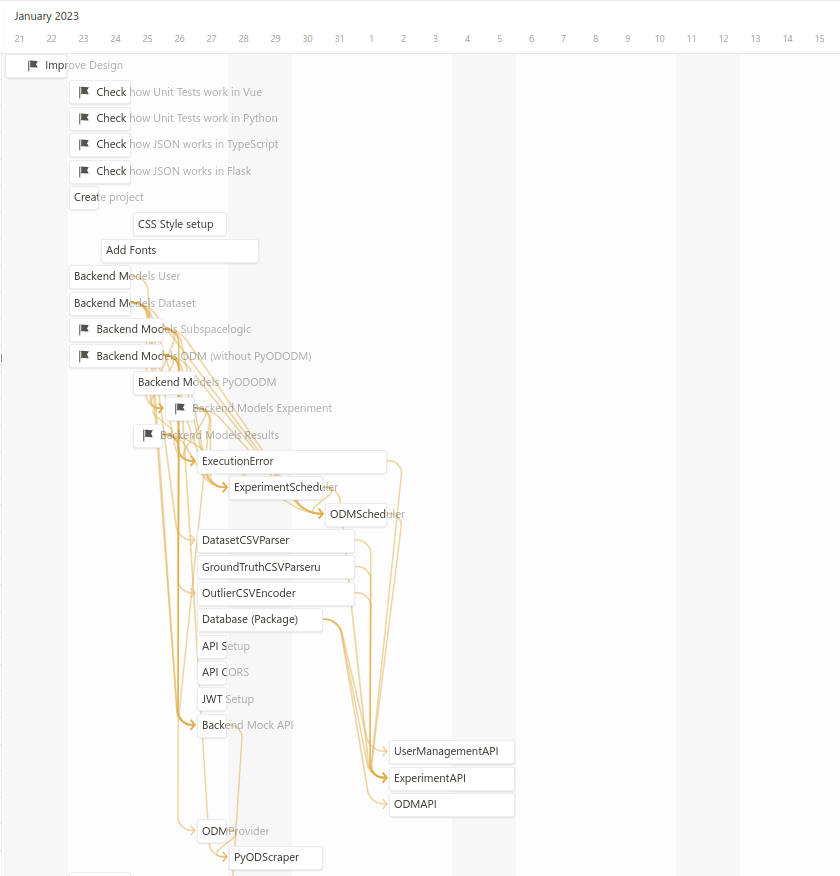
\includegraphics[width=\textwidth]{images/timeline-planned-backend.png}
    \caption{Planned timeline of the back-end tasks}
    \label{fig:timeline-planned-backend}
\end{figure}
\clearpage

\subsubsection*{Front-end}
\begin{figure}[!ht]
    \centering
    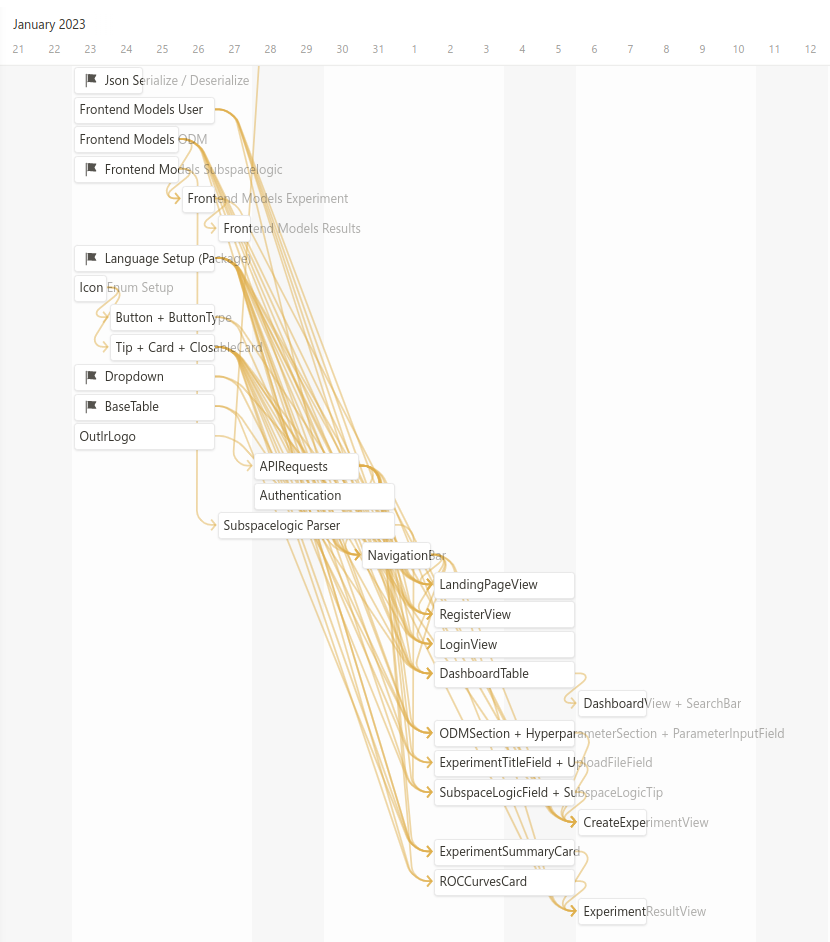
\includegraphics[width=\textwidth]{images/timeline-planned-frontend.png}
    \caption{Planned timeline of the front-end tasks}
    \label{fig:timeline-planned-frontend}
\end{figure}
\clearpage

\subsection{Actual timeline}
\subsubsection*{Back-end}
\begin{figure}[!ht]
    \centering
    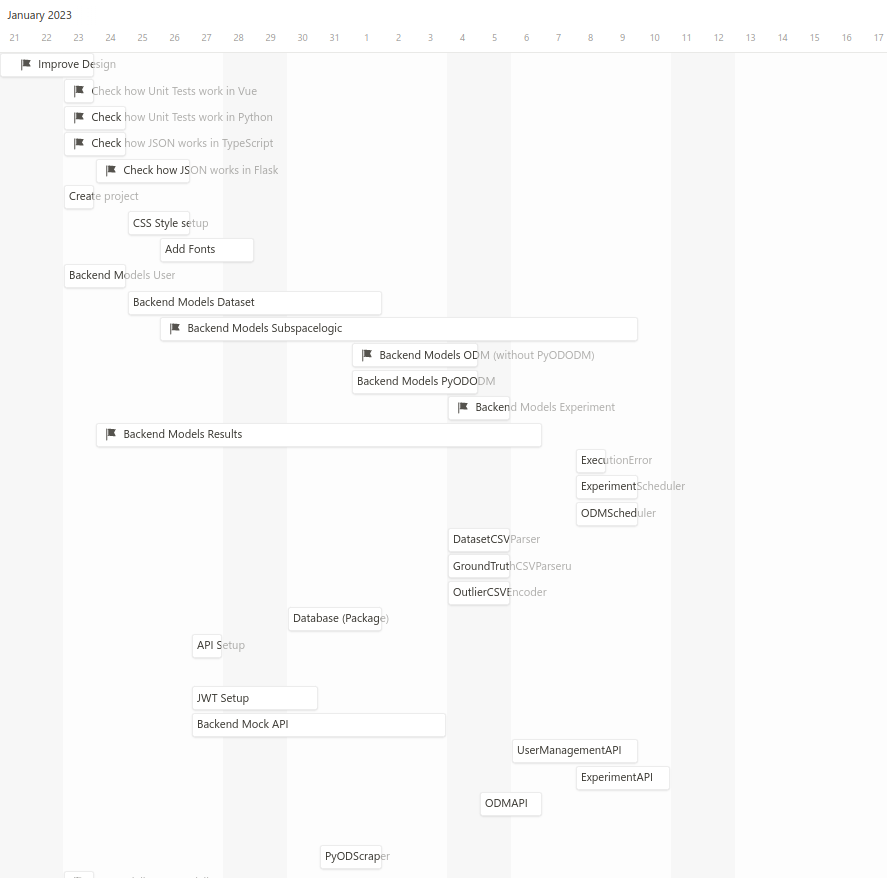
\includegraphics[width=\textwidth]{images/timeline-actual-backend.png}
    \caption{Actual timeline of the back-end tasks}
    \label{fig:timeline-actual-backend}
\end{figure}
\clearpage

\subsubsection*{Front-end}
\begin{figure}[!ht]
    \centering
    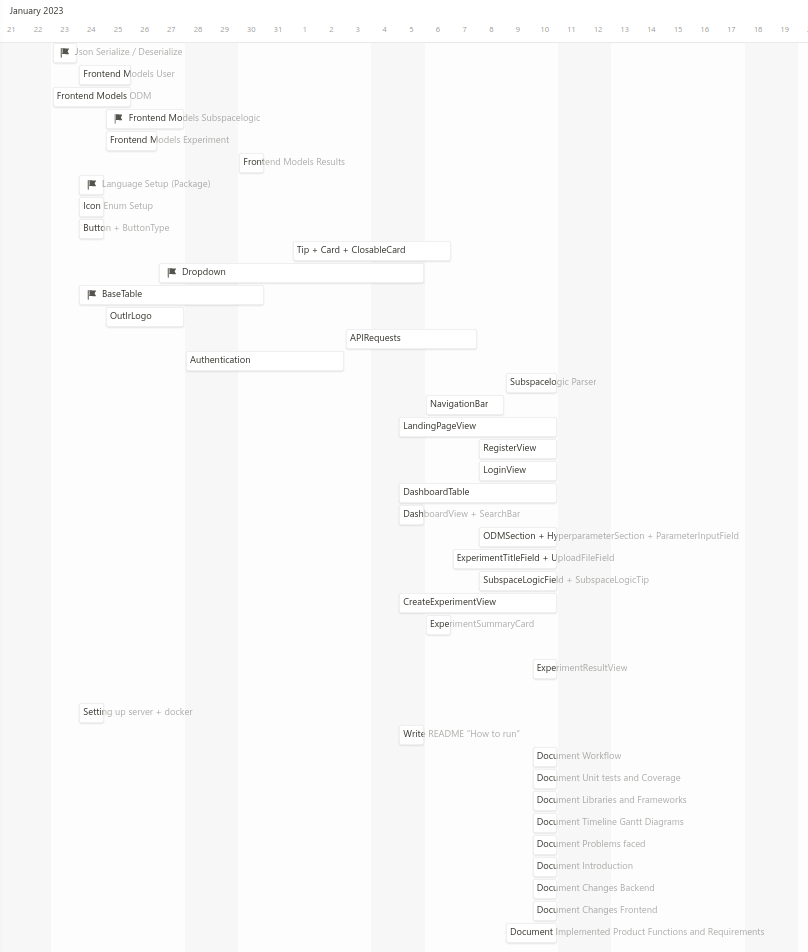
\includegraphics[width=\textwidth]{images/timeline-actual-frontend.png}
    \caption{Actual timeline of the front-end tasks}
    \label{fig:timeline-actual-frontend}
\end{figure}
\clearpage

\section{Statistics related to our implementation}
Lines of code in total: $\geq 6400$


\section{Overview of product functions, requirements defined in the Pflichtenheft}
\subsection*{Product Functions}
\subsubsection*{Mandatory}
Looking back at the software requirements specification we met our goal of providing all the defined mandatory product functions:
\begin{itemize}
    \item \textbf{FM1:} User Management: allowing a user to create an account, log in and logout
    \item \textbf{FM2:} Dashboard: providing an overview of all experiments
    \item \textbf{FM3:} Create Experiment: allowing a user to create an experiment, that is select an ODM, the hyperparameters for it and specify subspace logic for it.
    \item \textbf{FM4:} Run Experiment: run the experiment the user created
    \item \textbf{FM5:} Experiment Results: providing the user an overview of his run experiment
\end{itemize}
\subsubsection*{Optional}
As for the optional product functions we implemented:
\begin{itemize}
    \item \textbf{FO1}: providing the user with an appealing landing page 
\end{itemize}
However, we did not implement the other optional product functions, which were:
\begin{itemize}
    \item \textbf{FO2}: providing the user with an about us page giving users information about us
    \item \textbf{FO3} providing the user with a page, which compares the experiments the user selected before
\end{itemize}
The reason for not implementing these optional product functions was that implementing the other mandatory pages was time-consuming, not leaving us with enough time to work on the listed optional product functions.

\newpage
\subsection*{Requirements}
\subsubsection*{Mandatory}
As for the mandatory requirements we implemented all the defined mandatory requirements, which were: 
\begin{itemize}
    \item \textbf{RM1:} Allowing users to create an account
    \item \textbf{RM2:} Allowing users to log into their created accounts
    \item \textbf{RM3:} Allowing users to log out of their account
    \item \textbf{RM4:} Providing the user with a dashboard giving an overview of all experiments
    \item \textbf{RM5:} Allowing the user to click on the experiments in the dashboard, redirecting the user to the experiment's result
    \item \textbf{RM6:} Allowing users to name their experiment
    \item \textbf{RM7:} Allowing users to upload a dataset (.csv) for an experiment
    \item \textbf{RM8:} Allowing users to upload ground-truth to the provided dataset for an experiment
    \item \textbf{RM9:} Allowing users to select subspaces from the dataset, which shall be processed by the subspace logic
    \item \textbf{RM10:} Allowing users to specify subspace logic using logical or and logical and
    \item \textbf{RM11:} Allowing users to customize the hyperparameters of the ODM they selected
    \item \textbf{RM12:} Allowing users to select an ODM from a significant subset of the ODMs provided by PyOD
    \item \textbf{RM13:} Allowing users to a created experiment
    \item \textbf{RM14:} Allowing users to view the result of their experiment
    \item \textbf{RM15:} Allowing users to download a .csv file containing the indices of the detected outliers
    \item \textbf{RM16:} Outlr. is by default an English website
    \item \textbf{RM17:} Passwords are somewhat securely stored as the password are not stored in plain text but hashed. To achieve superior security these could be salted user-wise.
    \item \textbf{RM18:} Notifying the user of (unexpected) errors. The app mustn't crash when errors happen.
    \item \textbf{RM19:} "Outlr." is reliable and mature.
    \item \textbf{RM20:} "Outlr." is from our point of view easy to learn and provides efficient workflows.
    \item \textbf{RM21} For good resource management, "Outlr." releases all resources of an experiment after it is run.
    \item \textbf{RM22} "Outlr." is well documented and the code is easy to read.
    \item \textbf{RM23} From our point of view, "Outlr." has an appealing and modern design.
\end{itemize}
The optional requirements we implemented were:
\begin{itemize}
    \item \textbf{RO7:} Allowing the user to search experiments from his dashboard and clear the search term if wanted 
    \item \textbf{RO8:} Allowing the user to sort the dashboard by clicking on the table headers
    \item \textbf{RO13:} Allowing the user to nest logical operators in the subspace logic defined for an experiment
    \item \textbf{RO18:} Allowing the user to run experiments without passing a ground-truth file
\end{itemize}
However, we did not implement RO1-RO6, RO9-RO12, RO14-RO17, RO19-RO28. The reason for not implementing these optional requirements was that we did not have enough time to work on the listed optional requirements.


\newpage
\section{Libraries/Frameworks used}
Libraries and frameworks used on front-end side:
\begin{itemize}
    \item axios 1.2.3
    \item jest 29.4.2
    \item vue 3.2.45
    \item vue-i118n 9.2.2
    \item vue-router 4.1.6
    \item vuex 4.1.0
    \item vuex-persistedstate 4.1.0
\end{itemize}

Libraries and frameworks used on back-end side:
\begin{itemize}
    \item unittest
    \item Flask 2.2.2
    \item Flask-JWT-Extended 4.4.4
    \item Flask-CORS 3.0.10
    \item pandas 1.5.3
    \item pyod 1.0.7
    \item SQLALchemy 2.0.0
    \item psycopg2-binary 2.9.5
\end{itemize}
\newpage
\section{Overview of unit tests}
On front-end side;
\begin{itemize}
    \item Subspace Logic Parser tests
    \item Front-end model tests
    \begin{itemize}
        \item User tests
        \item Subspace tests
        \item Subspace logic tests
        \item Hyperparameter tests
        \item Experiment tests
    \end{itemize}
\end{itemize}

On back-end side:
\begin{itemize}
    \item Configuration (JWT secret key and database URL)test
    \item Experiment execution test
    \item Back-end model tests:
    \begin{itemize}
        \item User tests
        \item ODM tests
        \item Hyperparameter tests
        \item Experiment, Experiment result, Subspace tests (also checking database relations)
        \item PyOD ODM tests
        \item Subspace logic tests
        \item Tests, where objects are added to the database
        \item CSV functions tests
    \end{itemize}
\end{itemize}
\newpage
\section{Problems faced}
\begin{itemize}
    \item Difficulties setting up the CI/CD pipeline 
    \par Due to not having enough permissions on the SCC server and our Gitlab repository, our team faced difficulties setting up a proper CI/CD environment. This resulted in the postponed completion of some previously scheduled tasks.
    
    \item 
    Missing definition of JSONs
    \par
    We did not precisely define JSON requests and responses between the front-end and the back-end in the design phase. This was made up for in the implementation phase. Since the models have many references to each other defining the JSON structure was a difficult task. For these reasons, implementing the models took more time than expected.
    
    \item 
    Difficulties estimating how long tasks take to implement
    \par Tasks took longer than expected as can be deduced from the difference between the planned timeline and the timeline depicting the actual procedure

    \item
    Getting used to new tools\par
    Although \gls{python} and \gls{typescript} are relatively easy to learn it took the team some time to get used to. Additionally, working with frameworks like \gls{vue-js}, \gls{flask}, and \gls{SQLAlchemy} made it difficult to predict how long tasks take. Implementing the models using \gls{SQLAlchemy} took much more time than expected.
    
\end{itemize}
\newpage

\section{Design changes}

\subsection{General}
Since both \gls{python} and \gls{typescript} are not strictly object-oriented, we implemented some static utility classes or singleton classes from the class diagram by just writing the attributes and methods in the global scope.

\subsection{Back-end}
\package{backend.models.odm}
\code{ODM} is now an abstract class with an abstract \code{run\_odm} method.
\code{PyODM} implements \code{ODM} and calls the \gls{PyOD} library in the \code{run\_odm} method.
\code{check\_params} was removed.

\package{backend.models.experiment}
This package now contains the \code{Experiment}, \code{ExperimentResult}, \code{Subspace}, and \code{Outlier} classes.

\code{Subspace}s are now owned by the an \code{Experiment} directly instead of by an \code{ExperimentResult}. This is necessary because \code{Subspace}s exist before an \code{ExperimentResult} exists.

\code{Experiment} now has additional attributes:
\begin{itemize}
    \item \code{dataset\_name: str}
    \item \code{error\_json: dict | None} contains an error if the experiment execution failed
    \item \code{ground\_truth: np.NDArray | None} instead of \code{true\_outliers} contains the ground truth array of zeros and ones, is not stored in the database
\end{itemize}

\package{backend.execution}
No \code{QueueScheduler}s were implemented. Instead, a \code{CoroutineExperimentScheduler} and a \code{SequentialODMScheduler} were implemented.

\package{backend.parsers}
Moved all functions to module \code{util.data} and renamed them to the following:
\begin{itemize}
    \item \code{csv\_to\_dataset(name: str, dataset: str): Dataset}
    \item \code{csv\_to\_numpy\_array(csv: str): NDArray}
    \item \code{write\_list\_to\_csv(data: list[int], path: str): BytesIO}
\end{itemize}

\package{backend.api}
The endpoint \code{/experiment/upload-files} was created to upload the dataset and ground-truth files before experiment creation.\\
This was necessary as http only allows the content type to be either form-data or text/json. The former can contain raw files, the latter is used to give more information about the experiment to be created.

\package{backend.database}
Added more helper functions which were required in other places to \code{DatabaseAccess}.


\subsection{Front-end}

\package{frontend.components.basic}
The \code{Icon} enum was removed. Icons are now imported as a font.

\package{frontend.api}
\code{requestTokenCheck()} was renamed to \code{requestTokenIdentity()} and returns a JSON containing the username to the token if valid. If not valid as all other JSONs the JSON contains an error key.

To \code{AuthServices} the method
\code{intialValidityCheck()}, which, when the HTTP request has a valid token, sets the Vuex state, was added. Furthermore \code{validateUsername()} and \code{validatePassword()} were added.

\package{frontend.components.views.dashboard}
Added a \code{DashboardSortColumn} enum for sorting the dashboard table.

\package{frontend.components.views.createExperimentView}
The \code{ExperimentTitleField} vue component was removed and replaced by plain HTML code.

\package{frontend.models}
Because of the changes to our JSON files we had to implement different versions of the \code{fromJSONObject()} method with different function headers. And therefore we could not use the \code{JSONDeseializable} in all of our frontend modles.

\package{frontend.components.views}
The \code{LoginForm} and \code{RegisterForm} vue components also got removed and replaced by plain HTML code.

\newpage


\begin{appendices}

\printglossary
\printglossary[type=\acronymtype]\clearpage % print acronyms

% include appendix

\end{appendices}

\end{document}
